\documentclass[twoside]{book}

% Packages required by doxygen
\usepackage{calc}
\usepackage{doxygen}
\usepackage{graphicx}
\usepackage[utf8]{inputenc}
\usepackage{makeidx}
\usepackage{multicol}
\usepackage{multirow}
\usepackage{textcomp}
\usepackage[table]{xcolor}

% Font selection
\usepackage[T1]{fontenc}
\usepackage{mathptmx}
\usepackage[scaled=.90]{helvet}
\usepackage{courier}
\usepackage{amssymb}
\usepackage{sectsty}
\renewcommand{\familydefault}{\sfdefault}
\allsectionsfont{%
  \fontseries{bc}\selectfont%
  \color{darkgray}%
}
\renewcommand{\DoxyLabelFont}{%
  \fontseries{bc}\selectfont%
  \color{darkgray}%
}

% Page & text layout
\usepackage{geometry}
\geometry{%
  a4paper,%
  top=2.5cm,%
  bottom=2.5cm,%
  left=2.5cm,%
  right=2.5cm%
}
\tolerance=750
\hfuzz=15pt
\hbadness=750
\setlength{\emergencystretch}{15pt}
\setlength{\parindent}{0cm}
\setlength{\parskip}{0.2cm}
\makeatletter
\renewcommand{\paragraph}{%
  \@startsection{paragraph}{4}{0ex}{-1.0ex}{1.0ex}{%
    \normalfont\normalsize\bfseries\SS@parafont%
  }%
}
\renewcommand{\subparagraph}{%
  \@startsection{subparagraph}{5}{0ex}{-1.0ex}{1.0ex}{%
    \normalfont\normalsize\bfseries\SS@subparafont%
  }%
}
\makeatother

% Headers & footers
\usepackage{fancyhdr}
\pagestyle{fancyplain}
\fancyhead[LE]{\fancyplain{}{\bfseries\thepage}}
\fancyhead[CE]{\fancyplain{}{}}
\fancyhead[RE]{\fancyplain{}{\bfseries\leftmark}}
\fancyhead[LO]{\fancyplain{}{\bfseries\rightmark}}
\fancyhead[CO]{\fancyplain{}{}}
\fancyhead[RO]{\fancyplain{}{\bfseries\thepage}}
\fancyfoot[LE]{\fancyplain{}{}}
\fancyfoot[CE]{\fancyplain{}{}}
\fancyfoot[RE]{\fancyplain{}{\bfseries\scriptsize Generated on Wed Nov 22 2023 15\-:24\-:54 for C\-E\-L\-L\-G\-E\-O\-M\-E\-T\-R\-Y by Doxygen }}
\fancyfoot[LO]{\fancyplain{}{\bfseries\scriptsize Generated on Wed Nov 22 2023 15\-:24\-:54 for C\-E\-L\-L\-G\-E\-O\-M\-E\-T\-R\-Y by Doxygen }}
\fancyfoot[CO]{\fancyplain{}{}}
\fancyfoot[RO]{\fancyplain{}{}}
\renewcommand{\footrulewidth}{0.4pt}
\renewcommand{\chaptermark}[1]{%
  \markboth{#1}{}%
}
\renewcommand{\sectionmark}[1]{%
  \markright{\thesection\ #1}%
}

% Indices & bibliography
\usepackage{natbib}
\usepackage[titles]{tocloft}
\setcounter{tocdepth}{3}
\setcounter{secnumdepth}{5}
\makeindex

% Custom commands
\newcommand{\clearemptydoublepage}{%
  \newpage{\pagestyle{empty}\cleardoublepage}%
}


%===== C O N T E N T S =====

\begin{document}

% Titlepage & ToC
\pagenumbering{roman}
\begin{titlepage}
\vspace*{7cm}
\begin{center}%
{\Large C\-E\-L\-L\-G\-E\-O\-M\-E\-T\-R\-Y \\[1ex]\large 2.\-5.\-0 }\\
\vspace*{1cm}
{\large Generated by Doxygen 1.8.5}\\
\vspace*{0.5cm}
{\small Wed Nov 22 2023 15:24:54}\\
\end{center}
\end{titlepage}
\clearemptydoublepage
\tableofcontents
\clearemptydoublepage
\pagenumbering{arabic}

%--- Begin generated contents ---
\chapter{Hierarchical Index}
\section{Class Hierarchy}
This inheritance list is sorted roughly, but not completely, alphabetically\-:\begin{DoxyCompactList}
\item I\-Conditions\-Change\-Listener\begin{DoxyCompactList}
\item \contentsline{section}{C\-A\-L\-I\-C\-E\-:\-:multi\-Calibrator}{\pageref{classCALICE_1_1multiCalibrator}}{}
\end{DoxyCompactList}
\item Processor\begin{DoxyCompactList}
\item \contentsline{section}{C\-A\-L\-I\-C\-E\-:\-:multi\-Calibrator}{\pageref{classCALICE_1_1multiCalibrator}}{}
\end{DoxyCompactList}
\item T\-Object\begin{DoxyCompactList}
\item \contentsline{section}{T\-Convolution}{\pageref{classTConvolution}}{}
\end{DoxyCompactList}
\end{DoxyCompactList}

\chapter{Data Structure Index}
\section{Class List}
Here are the classes, structs, unions and interfaces with brief descriptions\-:\begin{DoxyCompactList}
\item\contentsline{section}{{\bf C\-A\-L\-I\-C\-E\-::multi\-Calibrator} \\*Processor to add P\-A\-R\-\_\-\-M\-U\-L\-T\-I to the event and calibrate the threshold }{\pageref{classCALICE_1_1multiCalibrator}}{}
\item\contentsline{section}{{\bf T\-Convolution} \\*R\-O\-O\-T class which generates the convolution of two functions }{\pageref{classTConvolution}}{}
\end{DoxyCompactList}

\chapter{Data Structure Documentation}
\section{C\-A\-L\-I\-C\-E\-:\-:Cell\-Description\-Processor Class Reference}
\label{classCALICE_1_1CellDescriptionProcessor}\index{C\-A\-L\-I\-C\-E\-::\-Cell\-Description\-Processor@{C\-A\-L\-I\-C\-E\-::\-Cell\-Description\-Processor}}


{\ttfamily \#include $<$Cell\-Description\-Processor.\-hh$>$}

Inheritance diagram for C\-A\-L\-I\-C\-E\-:\-:Cell\-Description\-Processor\-:\begin{figure}[H]
\begin{center}
\leavevmode
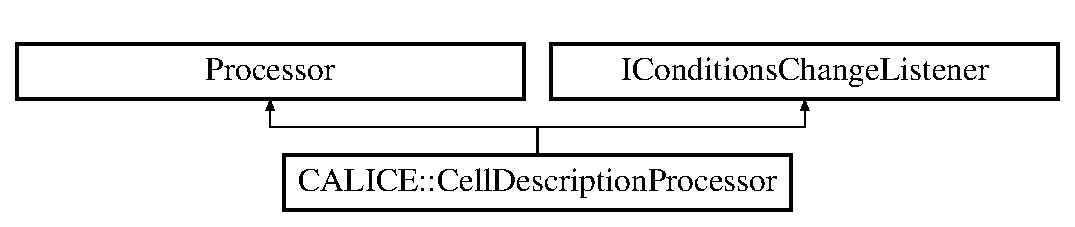
\includegraphics[height=2.000000cm]{classCALICE_1_1CellDescriptionProcessor}
\end{center}
\end{figure}
\subsection*{Public Member Functions}
\begin{DoxyCompactItemize}
\item 
virtual Processor $\ast$ {\bfseries new\-Processor} ()\label{classCALICE_1_1CellDescriptionProcessor_a5e862890c14f596f06bfbbfba622218d}

\item 
virtual void {\bfseries init} ()\label{classCALICE_1_1CellDescriptionProcessor_afc72f4838174f264a950b8c0fe00bcd3}

\item 
virtual void {\bfseries process\-Event} (L\-C\-Event $\ast$evt)\label{classCALICE_1_1CellDescriptionProcessor_a65bb278cc74192f8aa7c85aa388cdc14}

\item 
virtual void {\bfseries end} ()\label{classCALICE_1_1CellDescriptionProcessor_a35900c15f5190036b7329bbb99391161}

\item 
virtual void {\bfseries conditions\-Changed} (L\-C\-Collection $\ast$col)\label{classCALICE_1_1CellDescriptionProcessor_a9ecddf9e127f6891bfa08fd255fe046f}

\end{DoxyCompactItemize}
\subsection*{Static Public Member Functions}
\begin{DoxyCompactItemize}
\item 
static Mapped\-Container\\*
$<$ Cell\-Description $>$ $\ast$ {\bf get\-Cell\-Descriptions} (const std\-::string \&processor\-Name)
\end{DoxyCompactItemize}


\subsection{Detailed Description}
Processor that provides Cell\-Description for all cells.

The processor generates and updates a Mapped\-Container of Cell\-Description objects from the conditions data. To obtain the Mapped\-Collection in other processors use\-: \doxyref{Cell\-Description\-Processor\-::get\-Cell\-Descriptions}{p.}{classCALICE_1_1CellDescriptionProcessor_a6d60e618b66caabf2cee48b10e6c0ca1}( \char`\"{}cell\-Description processor name\char`\"{} )

\begin{DoxyParagraph}{processor parameters}
\begin{TabularC}{2}
\hline
steering file parameter name &description  \\\cline{1-2}
{\bfseries {\itshape  Detector\-Transformation }}&Name of the Detector\-Transformation collection \\\cline{1-2}
{\bfseries {\itshape  Mapping\-Processor\-Name }}&Name of the mapping processor that provides the necessary Mapper class \\\cline{1-2}
{\bfseries {\itshape  Module\-Connection }}&Name of the Module\-Connection collection \\\cline{1-2}
{\bfseries {\itshape  Module\-Description }}&Name of the Module\-Description collection \\\cline{1-2}
{\bfseries {\itshape  Module\-Location }}&Name of the Module\-Location collection \\\cline{1-2}
\end{TabularC}

\end{DoxyParagraph}
\begin{DoxyAuthor}{Author}
{\tt Benjamin.\-Lutz@desy.\-de} 
\end{DoxyAuthor}
\begin{DoxyVersion}{Version}
0.\-2 
\end{DoxyVersion}
\begin{DoxyDate}{Date}
November 2009 
\end{DoxyDate}


Definition at line 47 of file Cell\-Description\-Processor.\-hh.



\subsection{Member Function Documentation}
\index{C\-A\-L\-I\-C\-E\-::\-Cell\-Description\-Processor@{C\-A\-L\-I\-C\-E\-::\-Cell\-Description\-Processor}!get\-Cell\-Descriptions@{get\-Cell\-Descriptions}}
\index{get\-Cell\-Descriptions@{get\-Cell\-Descriptions}!CALICE::CellDescriptionProcessor@{C\-A\-L\-I\-C\-E\-::\-Cell\-Description\-Processor}}
\subsubsection[{get\-Cell\-Descriptions}]{\setlength{\rightskip}{0pt plus 5cm}Mapped\-Container$<$ Cell\-Description $>$ $\ast$ C\-A\-L\-I\-C\-E\-::\-Cell\-Description\-Processor\-::get\-Cell\-Descriptions (
\begin{DoxyParamCaption}
\item[{const std\-::string \&}]{processor\-Name}
\end{DoxyParamCaption}
)\hspace{0.3cm}{\ttfamily [static]}}\label{classCALICE_1_1CellDescriptionProcessor_a6d60e618b66caabf2cee48b10e6c0ca1}
static function to obtain cell description container


\begin{DoxyParams}[1]{Parameters}
\mbox{\tt in}  & {\em processor\-Name} & name of the \doxyref{Cell\-Description\-Processor}{p.}{classCALICE_1_1CellDescriptionProcessor} that takes care of this cell descriptions. \\
\hline
\end{DoxyParams}
\begin{DoxyReturn}{Returns}
pointer to the Mapped\-Container of Cell\-Descriptions 
\end{DoxyReturn}


Definition at line 22 of file Cell\-Description\-Processor.\-cc.



Referenced by C\-A\-L\-I\-C\-E\-::\-Correct\-Position\-Processor\-::init().



The documentation for this class was generated from the following files\-:\begin{DoxyCompactItemize}
\item 
Cell\-Description\-Processor.\-hh\item 
Cell\-Description\-Processor.\-cc\end{DoxyCompactItemize}

\section{C\-A\-L\-I\-C\-E\-:\-:Cell\-Neighbours\-Processor Class Reference}
\label{classCALICE_1_1CellNeighboursProcessor}\index{C\-A\-L\-I\-C\-E\-::\-Cell\-Neighbours\-Processor@{C\-A\-L\-I\-C\-E\-::\-Cell\-Neighbours\-Processor}}


{\ttfamily \#include $<$Cell\-Neighbours\-Processor.\-hh$>$}

Inheritance diagram for C\-A\-L\-I\-C\-E\-:\-:Cell\-Neighbours\-Processor\-:\begin{figure}[H]
\begin{center}
\leavevmode
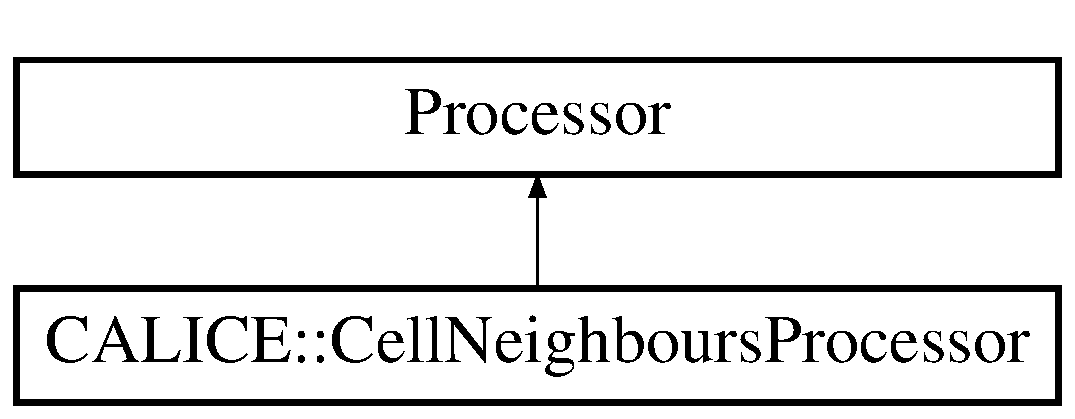
\includegraphics[height=2.000000cm]{classCALICE_1_1CellNeighboursProcessor}
\end{center}
\end{figure}
\subsection*{Public Member Functions}
\begin{DoxyCompactItemize}
\item 
virtual Processor $\ast$ {\bfseries new\-Processor} ()\label{classCALICE_1_1CellNeighboursProcessor_a5d8124b69f81b41bee91e95b96996b52}

\item 
virtual void {\bfseries init} ()\label{classCALICE_1_1CellNeighboursProcessor_acf6e2a5cc1d4592d1e49ab7f03b219e9}

\item 
virtual void {\bfseries process\-Event} (L\-C\-Event $\ast$evt)\label{classCALICE_1_1CellNeighboursProcessor_a07e3fc15bdb5db75f978e2bee0eb57a1}

\item 
virtual void {\bfseries end} ()\label{classCALICE_1_1CellNeighboursProcessor_adea30d7fda35bdfc4de28600f2ee40b3}

\end{DoxyCompactItemize}
\subsection*{Static Public Member Functions}
\begin{DoxyCompactItemize}
\item 
static Mapped\-Container\\*
$<$ Cell\-Neighbours $>$ $\ast$ {\bf get\-Neighbours} (const std\-::string \&processor\-Name)
\item 
static const std\-::string \& {\bfseries get\-Encoding\-String} (const std\-::string \&processor\-Name)\label{classCALICE_1_1CellNeighboursProcessor_ad963125fee09e610050846bace559a10}

\end{DoxyCompactItemize}


\subsection{Detailed Description}
Processor that provides cell neighbours information

To obtain the object in other processors use\-: \doxyref{Cell\-Neighbours\-Processor\-::get\-Neighbours}{p.}{classCALICE_1_1CellNeighboursProcessor_a9385534f41a3c60a91ba6cde01289f40}( \char`\"{}cell\-Neighbours processor name\char`\"{} )

\begin{DoxyParagraph}{processor parameters}
\begin{TabularC}{2}
\hline
steering file parameter name &description  \\\cline{1-2}
{\bfseries {\itshape  Mapping\-Processor\-Name }}&name of the mapping processor that provides the necessary Mapper class \\\cline{1-2}
\end{TabularC}

\end{DoxyParagraph}
\begin{DoxyAuthor}{Author}
{\tt Benjamin.\-Lutz@desy.\-de} 
\end{DoxyAuthor}
\begin{DoxyVersion}{Version}
0.\-1 
\end{DoxyVersion}
\begin{DoxyDate}{Date}
June 2009 
\end{DoxyDate}


Definition at line 41 of file Cell\-Neighbours\-Processor.\-hh.



\subsection{Member Function Documentation}
\index{C\-A\-L\-I\-C\-E\-::\-Cell\-Neighbours\-Processor@{C\-A\-L\-I\-C\-E\-::\-Cell\-Neighbours\-Processor}!get\-Neighbours@{get\-Neighbours}}
\index{get\-Neighbours@{get\-Neighbours}!CALICE::CellNeighboursProcessor@{C\-A\-L\-I\-C\-E\-::\-Cell\-Neighbours\-Processor}}
\subsubsection[{get\-Neighbours}]{\setlength{\rightskip}{0pt plus 5cm}Mapped\-Container$<$ Cell\-Neighbours $>$ $\ast$ C\-A\-L\-I\-C\-E\-::\-Cell\-Neighbours\-Processor\-::get\-Neighbours (
\begin{DoxyParamCaption}
\item[{const std\-::string \&}]{processor\-Name}
\end{DoxyParamCaption}
)\hspace{0.3cm}{\ttfamily [static]}}\label{classCALICE_1_1CellNeighboursProcessor_a9385534f41a3c60a91ba6cde01289f40}
static function to obtain a Mapped\-Container with cell neighbours


\begin{DoxyParams}[1]{Parameters}
\mbox{\tt in}  & {\em processor\-Name} & name of the \doxyref{Cell\-Neighbours\-Processor}{p.}{classCALICE_1_1CellNeighboursProcessor} that takes care of this Cell\-Neighbours. \\
\hline
\end{DoxyParams}
\begin{DoxyReturn}{Returns}
pointer to the Mapped\-Container including Cell\-Neighbours 
\end{DoxyReturn}


Definition at line 17 of file Cell\-Neighbours\-Processor.\-cc.



The documentation for this class was generated from the following files\-:\begin{DoxyCompactItemize}
\item 
Cell\-Neighbours\-Processor.\-hh\item 
Cell\-Neighbours\-Processor.\-cc\end{DoxyCompactItemize}

\section{C\-A\-L\-I\-C\-E\-:\-:Correct\-Position\-Processor Class Reference}
\label{classCALICE_1_1CorrectPositionProcessor}\index{C\-A\-L\-I\-C\-E\-::\-Correct\-Position\-Processor@{C\-A\-L\-I\-C\-E\-::\-Correct\-Position\-Processor}}


{\ttfamily \#include $<$Correct\-Position\-Processor.\-hh$>$}

Inheritance diagram for C\-A\-L\-I\-C\-E\-:\-:Correct\-Position\-Processor\-:\begin{figure}[H]
\begin{center}
\leavevmode
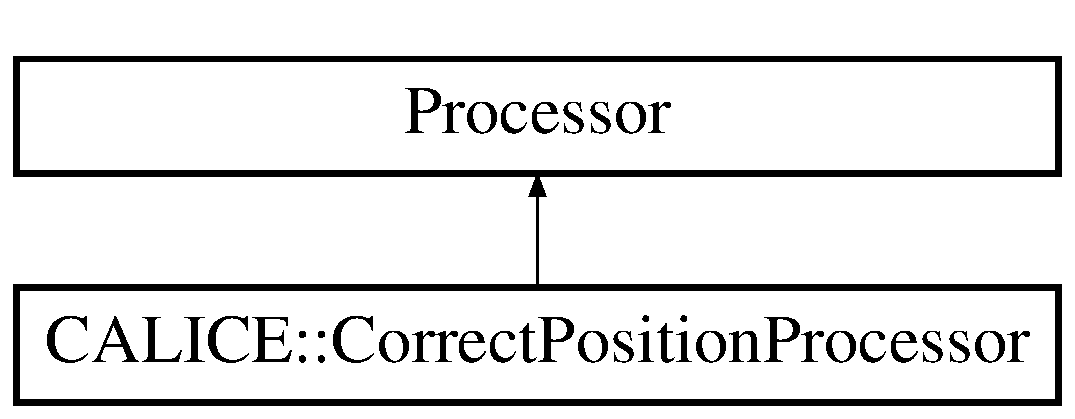
\includegraphics[height=2.000000cm]{classCALICE_1_1CorrectPositionProcessor}
\end{center}
\end{figure}
\subsection*{Public Member Functions}
\begin{DoxyCompactItemize}
\item 
virtual Processor $\ast$ {\bfseries new\-Processor} ()\label{classCALICE_1_1CorrectPositionProcessor_a2746de98b6d03b9eb77431df1016a062}

\item 
virtual void {\bf init} ()
\item 
virtual void {\bf process\-Event} (L\-C\-Event $\ast$evt)
\end{DoxyCompactItemize}
\subsection*{Protected Member Functions}
\begin{DoxyCompactItemize}
\item 
void {\bf create\-Sim\-Rec\-Relation} (L\-C\-Event $\ast$evt)
\item 
virtual void {\bf check\-Sim\-Rec\-Relation} (L\-C\-Event $\ast$evt)
\end{DoxyCompactItemize}


\subsection{Detailed Description}
Processor that generates a collection of Calorimeter\-Hits with corrected position.

\begin{DoxyParagraph}{processor parameters}
\begin{TabularC}{2}
\hline
steering file parameter name &description  \\\cline{1-2}
{\bfseries {\itshape  Cell\-Description\-Processor\-Name }}&name of the \doxyref{Cell\-Description\-Processor}{p.}{classCALICE_1_1CellDescriptionProcessor} that provides position information \\\cline{1-2}
{\bfseries {\itshape  Input\-Collection }}&name of the collection that contains the Calorimeter\-Hits to be corrected \\\cline{1-2}
{\bfseries {\itshape  Output\-Collection }}&name of the collection that will contain the corrected Calorimeter\-Hits \\\cline{1-2}
{\bfseries {\itshape  Scale\-Energy }}&scale factor for the energy of the hits \\\cline{1-2}
\end{TabularC}

\end{DoxyParagraph}
\begin{DoxyAuthor}{Author}
{\tt Benjamin.\-Lutz@desy.\-de} 
\end{DoxyAuthor}
\begin{DoxyVersion}{Version}
0.\-1 
\end{DoxyVersion}
\begin{DoxyDate}{Date}
June 2009 
\end{DoxyDate}


Definition at line 40 of file Correct\-Position\-Processor.\-hh.



\subsection{Member Function Documentation}
\index{C\-A\-L\-I\-C\-E\-::\-Correct\-Position\-Processor@{C\-A\-L\-I\-C\-E\-::\-Correct\-Position\-Processor}!check\-Sim\-Rec\-Relation@{check\-Sim\-Rec\-Relation}}
\index{check\-Sim\-Rec\-Relation@{check\-Sim\-Rec\-Relation}!CALICE::CorrectPositionProcessor@{C\-A\-L\-I\-C\-E\-::\-Correct\-Position\-Processor}}
\subsubsection[{check\-Sim\-Rec\-Relation}]{\setlength{\rightskip}{0pt plus 5cm}void C\-A\-L\-I\-C\-E\-::\-Correct\-Position\-Processor\-::check\-Sim\-Rec\-Relation (
\begin{DoxyParamCaption}
\item[{L\-C\-Event $\ast$}]{evt}
\end{DoxyParamCaption}
)\hspace{0.3cm}{\ttfamily [protected]}, {\ttfamily [virtual]}}\label{classCALICE_1_1CorrectPositionProcessor_a58578535a9a6c68351516650628c1c59}
Check the L\-C\-Relation between Mokka Sim\-Calorimeter\-Hits and reconstructed Calorimeter\-Hits 

Definition at line 276 of file Correct\-Position\-Processor.\-cc.

\index{C\-A\-L\-I\-C\-E\-::\-Correct\-Position\-Processor@{C\-A\-L\-I\-C\-E\-::\-Correct\-Position\-Processor}!create\-Sim\-Rec\-Relation@{create\-Sim\-Rec\-Relation}}
\index{create\-Sim\-Rec\-Relation@{create\-Sim\-Rec\-Relation}!CALICE::CorrectPositionProcessor@{C\-A\-L\-I\-C\-E\-::\-Correct\-Position\-Processor}}
\subsubsection[{create\-Sim\-Rec\-Relation}]{\setlength{\rightskip}{0pt plus 5cm}void C\-A\-L\-I\-C\-E\-::\-Correct\-Position\-Processor\-::create\-Sim\-Rec\-Relation (
\begin{DoxyParamCaption}
\item[{L\-C\-Event $\ast$}]{evt}
\end{DoxyParamCaption}
)\hspace{0.3cm}{\ttfamily [protected]}}\label{classCALICE_1_1CorrectPositionProcessor_a6cb567824d023f735791b2cb2bb3a399}
Create a collection of type L\-C\-Relation (relation between Mokka Sim\-Calorimeter\-Hits and reconstructed Calorimeter\-Hits), if the processor parameter Create\-Sim\-Rec\-Relation is true 

Definition at line 202 of file Correct\-Position\-Processor.\-cc.



Referenced by process\-Event().

\index{C\-A\-L\-I\-C\-E\-::\-Correct\-Position\-Processor@{C\-A\-L\-I\-C\-E\-::\-Correct\-Position\-Processor}!init@{init}}
\index{init@{init}!CALICE::CorrectPositionProcessor@{C\-A\-L\-I\-C\-E\-::\-Correct\-Position\-Processor}}
\subsubsection[{init}]{\setlength{\rightskip}{0pt plus 5cm}void C\-A\-L\-I\-C\-E\-::\-Correct\-Position\-Processor\-::init (
\begin{DoxyParamCaption}
{}
\end{DoxyParamCaption}
)\hspace{0.3cm}{\ttfamily [virtual]}}\label{classCALICE_1_1CorrectPositionProcessor_aa53c287405b06abca48790751f5aaab4}
Called at the begin of the job before anything is read. 

Definition at line 84 of file Correct\-Position\-Processor.\-cc.



References C\-A\-L\-I\-C\-E\-::\-Cell\-Description\-Processor\-::get\-Cell\-Descriptions(), and C\-A\-L\-I\-C\-E\-::\-Mapping\-Processor\-::get\-Mapper().

\index{C\-A\-L\-I\-C\-E\-::\-Correct\-Position\-Processor@{C\-A\-L\-I\-C\-E\-::\-Correct\-Position\-Processor}!process\-Event@{process\-Event}}
\index{process\-Event@{process\-Event}!CALICE::CorrectPositionProcessor@{C\-A\-L\-I\-C\-E\-::\-Correct\-Position\-Processor}}
\subsubsection[{process\-Event}]{\setlength{\rightskip}{0pt plus 5cm}void C\-A\-L\-I\-C\-E\-::\-Correct\-Position\-Processor\-::process\-Event (
\begin{DoxyParamCaption}
\item[{L\-C\-Event $\ast$}]{evt}
\end{DoxyParamCaption}
)\hspace{0.3cm}{\ttfamily [virtual]}}\label{classCALICE_1_1CorrectPositionProcessor_a8ec9f3ef853fb453faca1efd3b82d660}
Called for every event. 

Definition at line 119 of file Correct\-Position\-Processor.\-cc.



References create\-Sim\-Rec\-Relation().



The documentation for this class was generated from the following files\-:\begin{DoxyCompactItemize}
\item 
Correct\-Position\-Processor.\-hh\item 
Correct\-Position\-Processor.\-cc\end{DoxyCompactItemize}

\section{C\-A\-L\-I\-C\-E\-:\-:Mapping\-Processor Class Reference}
\label{classCALICE_1_1MappingProcessor}\index{C\-A\-L\-I\-C\-E\-::\-Mapping\-Processor@{C\-A\-L\-I\-C\-E\-::\-Mapping\-Processor}}


{\ttfamily \#include $<$Mapping\-Processor.\-hh$>$}

Inheritance diagram for C\-A\-L\-I\-C\-E\-:\-:Mapping\-Processor\-:\begin{figure}[H]
\begin{center}
\leavevmode
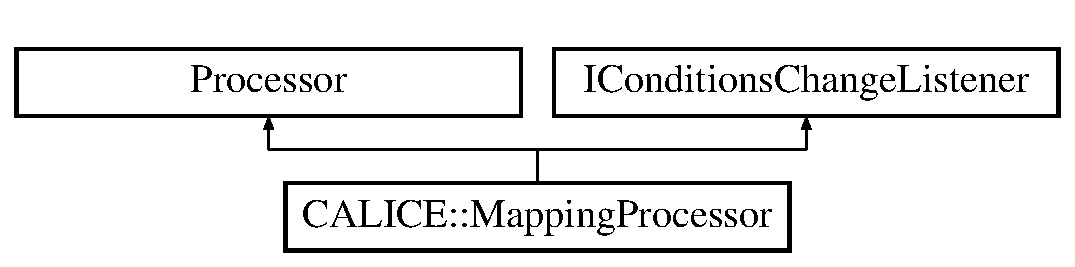
\includegraphics[height=2.000000cm]{classCALICE_1_1MappingProcessor}
\end{center}
\end{figure}
\subsection*{Public Member Functions}
\begin{DoxyCompactItemize}
\item 
virtual Processor $\ast$ {\bfseries new\-Processor} ()\label{classCALICE_1_1MappingProcessor_a7e51a6ba3abaf252cc5734ff9f192c43}

\item 
virtual void {\bfseries init} ()\label{classCALICE_1_1MappingProcessor_a8260b005f18c7d7dd26f78fca7c5f901}

\item 
virtual void {\bfseries process\-Event} (L\-C\-Event $\ast$evt)\label{classCALICE_1_1MappingProcessor_afd6f7befe771c3e261b3eb3033ccba0c}

\item 
virtual void {\bfseries end} ()\label{classCALICE_1_1MappingProcessor_abcc44104c737ea4dc9b8e40121391df4}

\end{DoxyCompactItemize}
\subsection*{Static Public Member Functions}
\begin{DoxyCompactItemize}
\item 
static const Mapper $\ast$ {\bf get\-Mapper} (const std\-::string \&processor\-Name)
\end{DoxyCompactItemize}


\subsection{Detailed Description}
Processor that provides a C\-A\-L\-I\-C\-E Mapper object.

The processor generates and updates a C\-A\-L\-I\-C\-E Mapper object from the conditions data. To obtain the object in other processors use\-: \doxyref{Mapping\-Processor\-::get\-Mapper}{p.}{classCALICE_1_1MappingProcessor_a0ab9895933daf9f277135afb8aa24376}( \char`\"{}mapping processor name\char`\"{} )

\begin{DoxyAuthor}{Author}
{\tt Benjamin.\-Lutz@desy.\-de} 
\end{DoxyAuthor}
\begin{DoxyVersion}{Version}
0.\-2 
\end{DoxyVersion}
\begin{DoxyDate}{Date}
November 2009 
\end{DoxyDate}


Definition at line 32 of file Mapping\-Processor.\-hh.



\subsection{Member Function Documentation}
\index{C\-A\-L\-I\-C\-E\-::\-Mapping\-Processor@{C\-A\-L\-I\-C\-E\-::\-Mapping\-Processor}!get\-Mapper@{get\-Mapper}}
\index{get\-Mapper@{get\-Mapper}!CALICE::MappingProcessor@{C\-A\-L\-I\-C\-E\-::\-Mapping\-Processor}}
\subsubsection[{get\-Mapper}]{\setlength{\rightskip}{0pt plus 5cm}const Mapper $\ast$ C\-A\-L\-I\-C\-E\-::\-Mapping\-Processor\-::get\-Mapper (
\begin{DoxyParamCaption}
\item[{const std\-::string \&}]{processor\-Name}
\end{DoxyParamCaption}
)\hspace{0.3cm}{\ttfamily [static]}}\label{classCALICE_1_1MappingProcessor_a0ab9895933daf9f277135afb8aa24376}
static function to obtain mapper


\begin{DoxyParams}[1]{Parameters}
\mbox{\tt in}  & {\em processor\-Name} & name of the \doxyref{Mapping\-Processor}{p.}{classCALICE_1_1MappingProcessor} that takes care of this Mapper. \\
\hline
\end{DoxyParams}
\begin{DoxyReturn}{Returns}
pointer to the mapper 
\end{DoxyReturn}


Definition at line 24 of file Mapping\-Processor.\-cc.



Referenced by C\-A\-L\-I\-C\-E\-::\-Correct\-Position\-Processor\-::init().



The documentation for this class was generated from the following files\-:\begin{DoxyCompactItemize}
\item 
Mapping\-Processor.\-hh\item 
Mapping\-Processor.\-cc\end{DoxyCompactItemize}

%--- End generated contents ---

% Index
\newpage
\phantomsection
\addcontentsline{toc}{part}{Index}
\printindex

\end{document}
